\documentclass[11pt]{article}

\usepackage{amsmath,amssymb,amsfonts}
\usepackage{dsfont}
\usepackage{listings}
\usepackage{xcolor}
\usepackage{graphicx}
\usepackage{bbm}
\usepackage{float}
\usepackage{hyperref}



\definecolor{codegreen}{rgb}{0,0.6,0}
\definecolor{codegray}{rgb}{0.5,0.5,0.5}
\definecolor{codepurple}{rgb}{0.58,0,0.82}
\definecolor{backcolour}{rgb}{0.95,0.95,0.92}
\lstdefinestyle{mystyle}{
    backgroundcolor=\color{backcolour},
    commentstyle=\color{codegreen},
    keywordstyle=\color{magenta},
    numberstyle=\tiny\color{codegray},
    stringstyle=\color{codepurple},
    basicstyle=\ttfamily\footnotesize,
    breakatwhitespace=false,
    breaklines=true,
    captionpos=b,
    keepspaces=true,
    numbers=left,
    numbersep=5pt,
    showspaces=false,
    showstringspaces=false,
    showtabs=false,
    tabsize=2
}

\setlength{\topmargin}{-.5in} \setlength{\textheight}{9.25in}
\setlength{\oddsidemargin}{0in} \setlength{\textwidth}{6.8in}

%\newcommand*{\SOLVE}{}%

\renewcommand{\vec}[1]{\mbox{\boldmath$#1$}}
\newcommand{\mm}[1]{\mathbf{#1}}

\newcounter{ProblemNum}
\newcounter{SubProblemNum}[ProblemNum]

\renewcommand{\theProblemNum}{\arabic{ProblemNum}}
\renewcommand{\theSubProblemNum}{\alph{SubProblemNum}}

\newcommand*{\anyproblem}[1]{\section*{#1}}
\newcommand*{\problem}[1]{\stepcounter{ProblemNum} %
   \anyproblem{Problem \theProblemNum \; (#1 points)}}
\newcommand*{\soln}[1]{\subsection*{#1}}
\newcommand*{\solution}{\soln{Solution}}
\newenvironment{solutions}
  {\section[Solution]{\textcolor{red}{Solution}}\color{red}}
  {\normalcolor}
\renewcommand*{\part}{\stepcounter{SubProblemNum} %
  \soln{Part (\theSubProblemNum)}}
\renewcommand{\theenumi}{(\alph{enumi})}
\renewcommand{\labelenumi}{\theenumi}
\renewcommand{\theenumii}{\roman{enumii}}
\let\endsection\relax
\let\endsubsection\relax

\graphicspath{
{.}
}
\lstset{style=mystyle}

\begin{document}

\Large
\noindent{\bf CS4851/6851 IDL: Homework 2 \hfill \today}
\medskip\hrule

\vspace{20pt}

Note: All coding problems to be submited with Github Link. Do not Upload the files/folder. Use git commands only.

Note: this is the distribution of questions:
\begin{enumerate}
  \item Question 1 to Question6: Required for everyone.
  \item Question 7 - Question 8: Required only for Graduate Students
  \item Question 9- Question 10: Bonus marks
\end{enumerate}


\problem{5} We covered Automatic Differentiation in class. Consider the following function:

\begin{equation}
  f(x, y, z)=   \frac{1}{3} (x_1x_2\sin(x_3) + exp^{x_1x_2})
\end{equation}

\begin{enumerate}
  \item Draw a computation graph for this function.
  \item List the detailed computation steps (the trace) for forward and backward mode of AD. Provide your answers the same way we did in class, by using notations like: 
      \begin{equation}
        v_{-2}, v_{-1}, v_{0}, v_{1}, v_{2}
      \end{equation}

  to get you started:
  \begin{equation}
    v_{-2} = 1, \dot{v}_{-2} = \frac{\partial{v_{-2}}}{\partial{x_{-2}}} = 0
  \end{equation}

  Provide all the steps like this and values for other nodes in computation graph.
\end{enumerate}

\problem{5} Select the correct option.Accuracy is probably the most commonly used metric in the most common type of Deep 
learning problems:

\begin{enumerate}
  \item Accuracy is very easy to interpret and is aligned on what you want to measure.
  \item Accuracy is differential and can be used to directly in gradient based optimisation process
  \item We want accuracy to count every error as equal.
  \item If the number of sample is similar, we cannot make any mistake on the less populated category.
\end{enumerate}


\problem{10} You are working as a Machine Learning Engineer in Metflix Inc. You are building a model to classify users who watch a lot of movies in Ultiverse. What metrics will you choose to evaluate your model?

\problem{10} Which method is used involved in numerical optimization of an appropriate selection of model criterion? How do you define the error of such estimator? 

\problem{10} 
\begin{figure}[H]
  \begin{center}
    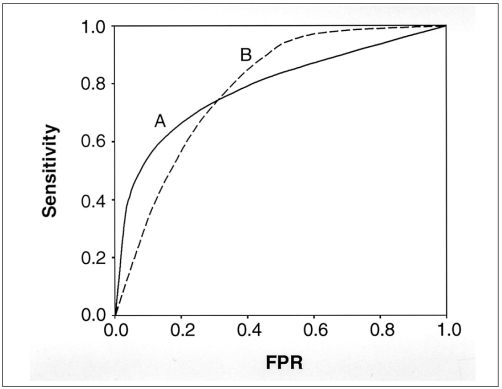
\includegraphics[width=1.0\textwidth]{Two-ROC-curves-A-and-B-with-equal-area-under-the-ROC-curve-However-these-two-ROC.png}
  \end{center}
  \caption{Two curves with equal area under the ROC curve}
\end{figure}

In the above figure we have two ROC curve (A and B) which has the same area under the curve. Which one is better among these two and what governs the area under the curve?


\problem{20}
why is it that technically we're looking for gradient with respect to $W_i$, where $W_i$ is the linear transform (or parameter) matrix (tensor) for each layer. Yet, we are computing $\frac{d(loss)}{d(x)}$, where $x$ is the input. How come?

\vspace{20pt}
\noindent\rule[0.5ex]{0.45\linewidth}{1pt} Bonus for undergraduates beyond this line

\problem{20} Compare the following metrics and explain which one is better.

\begin{enumerate}
  \item ROC and AUC 
    \begin{figure}[H]
      \begin{center}
        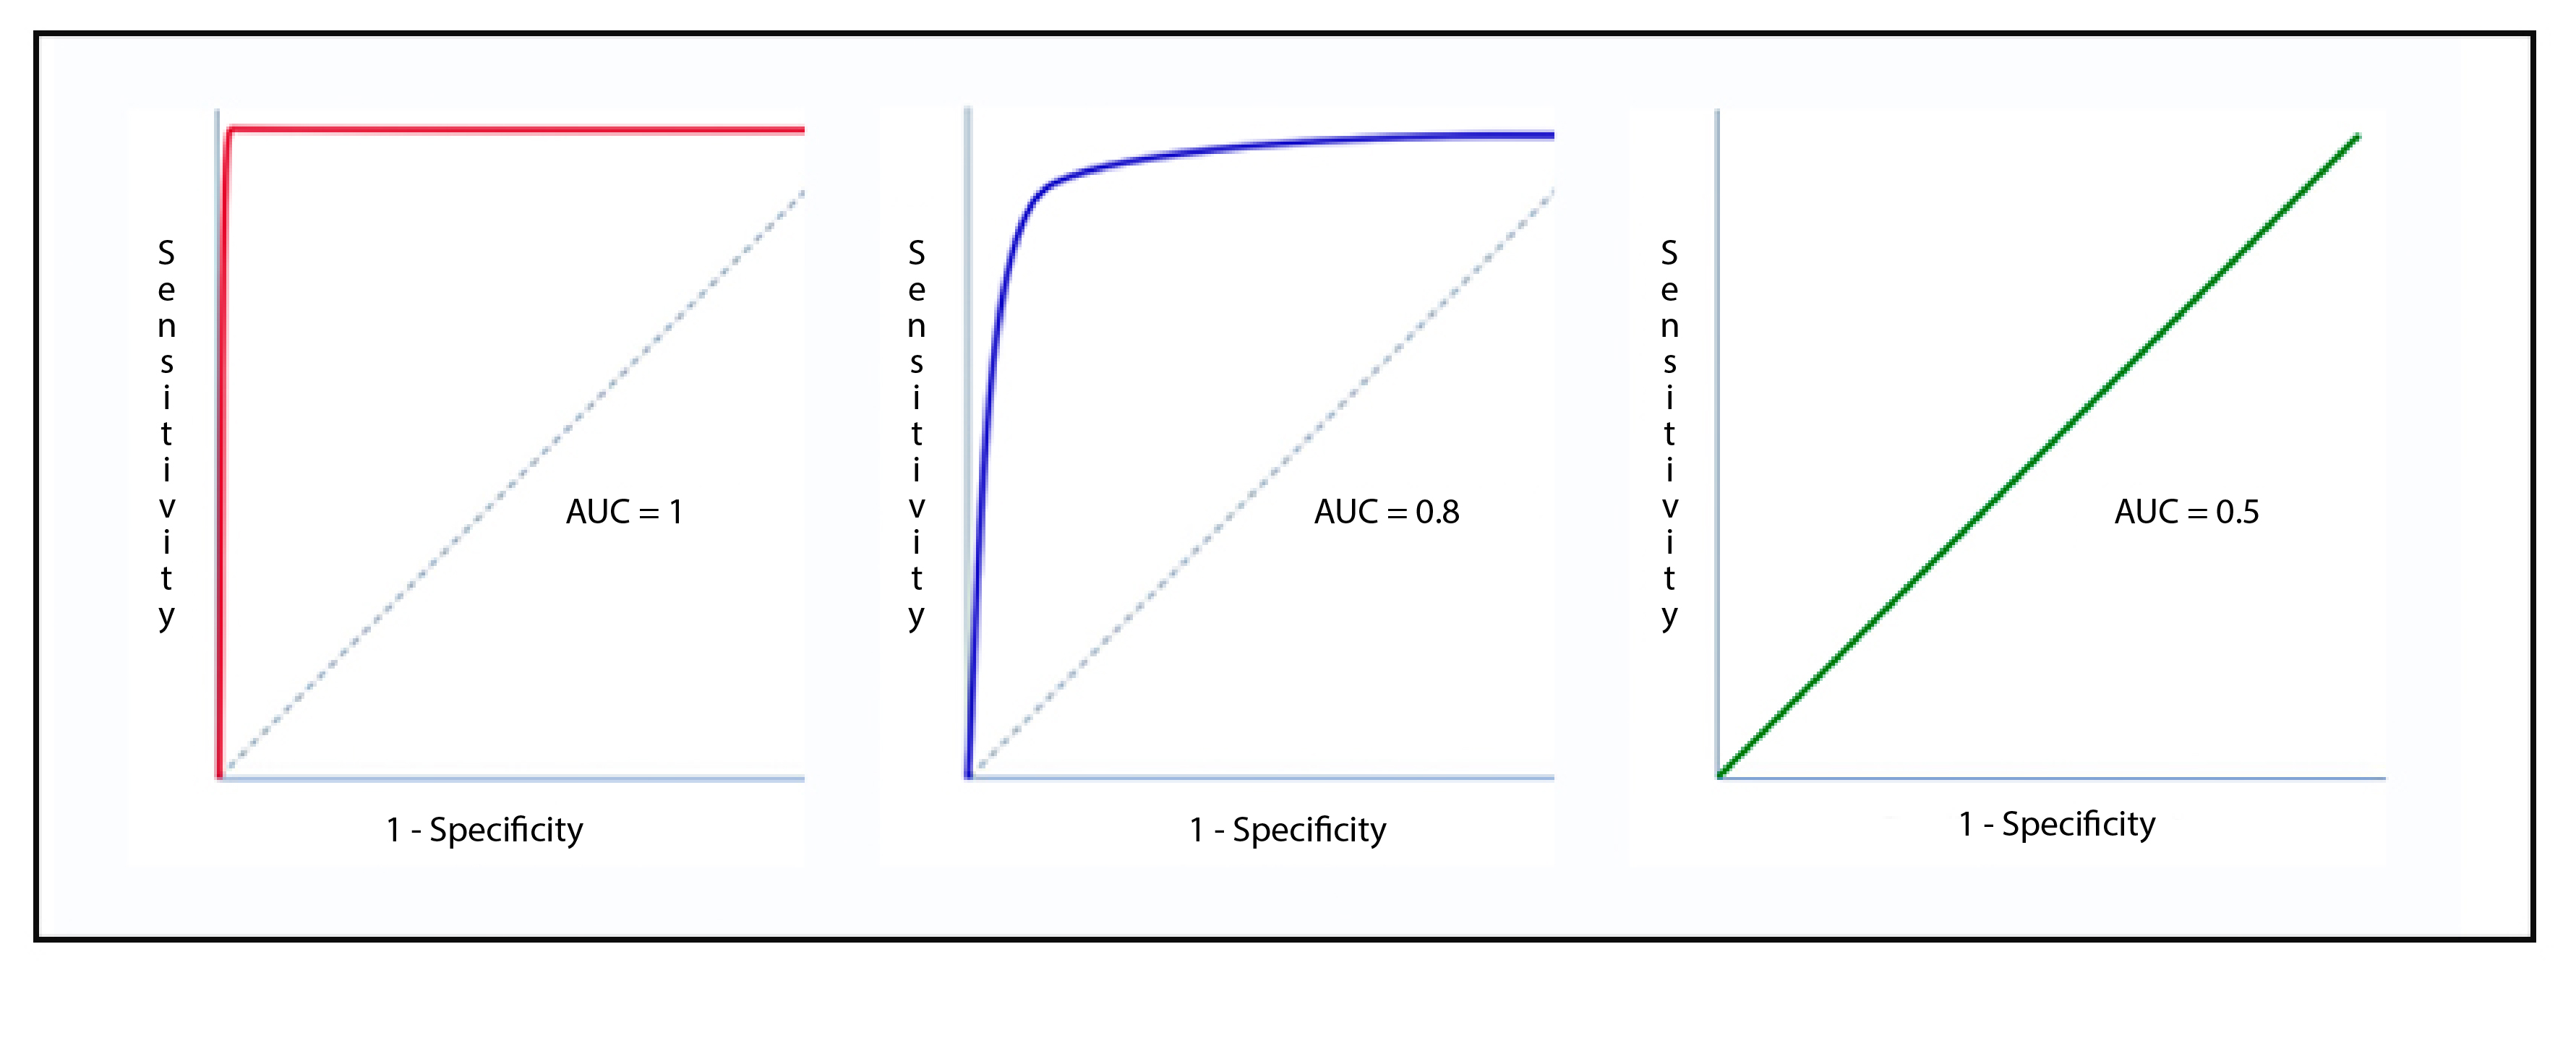
\includegraphics[width=1.0\textwidth]{AUC_curve.jpeg}
      \end{center}
      \caption{Accuracy}
    \end{figure}
  \item For the same figure, explain relevance to True Positive Rate (TPR) and False Positive Rate (FPR)
\end{enumerate}


\noindent\rule[0.5ex]{\linewidth}{1pt}
% \vspace{2px}
\end{document}

%%% Local Variables:
%%% mode: latex
%%% TeX-master: t
%%% End:

